% 附录 X：辐射输运与辐射损失（v1.22.0 新增）
% 数值唯一来源：tools/calc/appX_calc.py -> tools/calc/appX_calc.txt（正文数字的唯一来源；检查项 P29）
% 时间/功率单位写成 s、MW，避免中文字符进入数学字体；全部数字可用仓库脚本复算。
% 版权口径：只借鉴经典教材与文献的物理结论、公式形式与题型；文字、数值与表格自拟并独立复算。
% 本书不列 DOI，只给书名、作者、年份、卷期页。
% 分工：M 管加热与电流驱动，N 管边界与瞬态热负荷，S 管约束，U 管增益与点火，
%       V 管运行空间什么时候被撞破，W 管快粒子与 alpha 粒子本身；
%       本附录管能量的另一条出口——辐射把能量带走了多少、带去了哪里。

\section{三种辐射机制：先算光学薄上限}
\label{sec:app-x-three}

前面几本账把能量的来路算完了。附录 M 算加热与电流驱动，附录 S 把约束写成一个
$\tau_E$，附录 U 把增益算到电功率，附录 W 追着 3.5 MeV 的 alpha 粒子看它把能量
交给了谁。但能量还有一条出口一直没算：\textbf{辐射}。附录 U 的功率账里有一行「辐射损失」，
附录 N 算壁负荷时只算了传导与对流。本节把三种辐射机制在\textbf{光学薄假设}下各算一遍，
只看量级，不涉及输运方程。

工作点沿用 D1：$n_e=10^{20}\ \mathrm{m^{-3}}$、$T_e=9.194\ \mathrm{keV}$、
$B=5.3\ \mathrm{T}$、$a=2.0\ \mathrm{m}$、$R=6.2\ \mathrm{m}$、
$V=832.2\ \mathrm{m^3}$、$Z_{\mathrm{eff}}=2$，取
$P_{\mathrm{fus}}=556.5\ \mathrm{MW}$、$P_\alpha=111.3\ \mathrm{MW}$、
热储能 $W_{\mathrm{th}}=371.4\ \mathrm{MJ}$。

三种机制的光学薄功率密度分别是：轫致辐射
\begin{equation}
P_{\mathrm{br}} = 5.35\times10^{-37}\,Z_{\mathrm{eff}}\,n_e^2\sqrt{T_e\,[\mathrm{keV}]}
= 3.2444\times10^{4}\ \mathrm{W\,m^{-3}} = 32.444\ \mathrm{kW\,m^{-3}},
\label{eq:app-x-brnum}
\end{equation}
回旋辐射（单电子 Larmor 功率乘以电子密度）
\begin{equation}
P_{\mathrm{cyc}}^{\mathrm{thin}} = n_e\,\frac{4}{3}\sigma_T c\,\beta_\perp^2\,u_B
= 1.0695\times10^{6}\ \mathrm{W\,m^{-3}} = 1.0695\ \mathrm{MW\,m^{-3}},
\label{eq:app-x-cycthin}
\end{equation}
线辐射（钨，$n_W/n_e=10^{-5}$）
\begin{equation}
P_{\mathrm{line}} = n_e n_W L_W = 10^{3}\ \mathrm{W\,m^{-3}} = 1\ \mathrm{kW\,m^{-3}}.
\label{eq:app-x-line}
\end{equation}
式 \eqref{eq:app-x-cycthin} 里 $u_B=B^2/(2\mu_0)=1.11767\times10^{7}\ \mathrm{J\,m^{-3}}$
是磁能密度，$\beta_\perp^2=2T_e/(m_ec^2)=0.035984$ 是电子的无量纲热速度平方，
$\sigma_T$ 是 Thomson 截面。式 \eqref{eq:app-x-line} 里的冷却率系数 $L_W$ 取
$10^{-32}\ \mathrm{W\,m^3}$，这是\textbf{声明}的量级值，理由与适用范围写在 X.5。

\begin{table}[htbp]
\centering
\small
\begin{tabular}{p{2.5cm}p{3.1cm}p{2.9cm}p{4.6cm}}
\toprule
机制 & 光学薄功率密度 & 全等离子体 & 备注 \\
\midrule
轫致辐射 & $32.444\ \mathrm{kW\,m^{-3}}$ & $27.00\ \mathrm{MW}$ & 连续谱，光子能量 $\sim T_e$ \\
回旋辐射 & $1.0695\ \mathrm{MW\,m^{-3}}$ & $890.01\ \mathrm{MW}$ & 光学薄值\textbf{大于} $P_{\mathrm{fus}}$ \\
线辐射 & $1\ \mathrm{kW\,m^{-3}}$ & $0.8322\ \mathrm{MW}$ & 只算钨，$n_W/n_e=10^{-5}$ \\
\bottomrule
\end{tabular}
\caption{三种辐射机制的光学薄量级。第三列是把功率密度乘 $V$ 的结果。
第二行的数字故意留着不合物理的结论，X.4 会解释它为什么错。}
\label{tab:app-x-channel}
\end{table}

表 \ref{tab:app-x-channel} 第二行给出一个不可能的数：回旋辐射的光学薄估算为
$890.01\ \mathrm{MW}$，是聚变功率 $556.5\ \mathrm{MW}$ 的 $1.5993$ 倍。如果这是真的，
任何托卡马克都不可能点火：反应堆单靠回旋辐射就损失掉一点六倍的聚变功率。
这个「不可能」不是算错了，而是\textbf{光学薄假设用错了地方}：
回旋辐射在磁化等离子体里是\textbf{共振}过程，等离子体对它是光学厚的，
绝大部分辐射在原地就被重新吸收回去。所以正确的做法是给两个边界：
光学薄上限（式 \eqref{eq:app-x-cycthin}）与黑体上限（X.4），真值夹在中间。

\begin{tip}{先算上限，再谈输运}{tip-app-x-upperbound}
遇到一个新的损失通道，不要一上来就写输运方程。先问一句：\textbf{如果它全部逃逸，能带走多少？}
这个上限不需要任何输运知识，只需要一个发射率公式。上限算出来就两种情况：
比主账小很多（那它不重要，可以走开）；比主账还大（那它一定被再吸收，
接下来要算的才是输运）。本附录三种辐射正好把两种情况都碰到了。
\end{tip}

{\footnotesize
\textbf{出处：}三种机制的划分与轫致辐射公式参照 Wesson \emph{Tokamaks}（第 4 版，2011，
第 2 章）与 NRL \emph{Plasma Formulary}（2018，辐射节）。
光学薄与光学厚的判据参照
Rybicki \& Lightman \emph{Radiative Processes in Astrophysics}（1979，第 1、5 章）。
}

\section{光学薄还是光学厚：轫致辐射为什么逃得掉}
\label{sec:app-x-opacity}

辐射是不是损失，取决于一个无量纲数：光学深度
\begin{equation}
\tau_\nu = \int \alpha_\nu \diff l \;\approx\; \alpha_\nu L,
\label{eq:app-x-optdepth}
\end{equation}
其中 $\alpha_\nu$ 是吸收系数，$L$ 是弦长。$\tau_\nu\ll1$ 时光子一路跑出去，
发射率就是损失率；$\tau_\nu\gg1$ 时等离子体自己就是黑体，
逃逸功率由表面温度决定，与发射率无关。

自由-自由（逆轫致）吸收系数在经典文献里常写成 cgs 形式
\begin{equation}
\alpha_\nu^{\mathrm{ff}} = 3.7\times10^{8}\,
Z^2 n_e n_i\,T^{-1/2}\nu^{-3}
\left(1-e^{-h\nu/k_BT}\right)\ \mathrm{cm^{-1}},
\label{eq:app-x-ffabs}
\end{equation}
其中 $T$ 用 K、$\nu$ 用 Hz、密度用 $\mathrm{cm^{-3}}$。在 D1 工作点上，
$T=1.0669\times10^{8}\ \mathrm{K}$，取回旋频率 $\nu=f_{ce}=1.4836\times10^{11}\ \mathrm{Hz}$
（式 \eqref{eq:app-x-cyclfreq}），指数因子 $h\nu/k_BT=6.6736\times10^{-8}$，
于是
\begin{equation}
\alpha_{ff} = 1.46411\times10^{-6}\ \mathrm{m^{-1}},
\qquad
\tau_{ff} = \alpha_{ff}\,(2a) = 5.85642\times10^{-6}.
\label{eq:app-x-tauff}
\end{equation}
$\tau_{ff}$ 比 $1$ 小五个数量级：\textbf{托卡马克对自身的轫致辐射永远是光学薄的}，
发出的每一个轫致光子几乎都会跑到壁上。等价的说法是平均自由程
$1/\alpha_{ff}=6.8301\times10^{5}\ \mathrm{m}$，也就是 $683\ \mathrm{km}$，
是装置尺度 $4\ \mathrm{m}$ 的 $1.7075\times10^{5}$ 倍。

\begin{table}[htbp]
\centering
\small
\begin{tabular}{p{2.6cm}p{3.4cm}p{3.4cm}p{3.2cm}}
\toprule
判据 & 光学薄 $\tau\ll1$ & 光学厚 $\tau\gg1$ & 本工作点归属 \\
\midrule
逃逸份额 & 接近 $1$ & $\sim1/\tau$，可以极小 & 轫致辐射：光学薄 \\
损失由谁决定 & 发射率 & 表面温度（黑体） & 轫致：发射率 \\
吸收类型 & 自由-自由（非共振） & 共振（回旋谐波） & 回旋：共振 \\
可否只看发射率 & 可以 & 不可以 & 回旋：不可以 \\
\bottomrule
\end{tabular}
\caption{两种极限的判据与归属。把这个表当成查表用：遇到任何一条新的辐射通道，
先判断它落在哪一列，再决定要不要算输运。}
\label{tab:app-x-opacity}
\end{table}

轫致辐射与回旋辐射的差别不在发射率，而在\textbf{吸收是不是共振的}。
式 \eqref{eq:app-x-ffabs} 是自由-自由过程，任何频率都能发生，所以极其微弱；
回旋吸收只在 $\omega\approx n\omega_{ce}$ 的窄带上发生，窄带上的吸收系数大得多的多，
光学深度因此远大于 $1$。同一块等离子体，对一种是透明的，对另一种是不透明的。

\begin{tip}{辐射是不是损失，由输运决定}{tip-app-x-transport}
「等离子体发出多少辐射」与「等离子体损失多少能量」是两个不同的问题。
前者是发射率，后者是发射率乘以逃逸份额。在光学厚的情形里，
逃逸份额可以小到百万分之一，这时\textbf{发射率算得再准也没有意义}——
真正决定损失的是表面温度与再吸收。看文献里的辐射损失数字时，
先确认它说的是 emission 还是 loss。
\end{tip}

{\footnotesize
\textbf{出处：}光学深度与自由-自由吸收的具体形式参照 Rybicki \& Lightman
\emph{Radiative Processes in Astrophysics}（1979，式 5.18 一带）。
共振吸收与回旋辐射的输运处理参照 Bornatici 等（1983）\emph{Nucl.\ Fusion} \textbf{23}, 1153。
}

\section{轫致辐射：为什么它总是主要损失}
\label{sec:app-x-brems}

轫致辐射是电子在离子库仑场里被偏转时发出的连续谱。对麦克斯韦分布的电子，
功率密度可以写成式 \eqref{eq:app-x-brnum} 的紧凑形式：
\begin{equation}
P_{\mathrm{br}} = 5.35\times10^{-37}\,Z_{\mathrm{eff}}\,n_e^2\,
\sqrt{T_e\,[\mathrm{keV}]}\ \ \mathrm{W\,m^{-3}}.
\label{eq:app-x-br}
\end{equation}
在 D1 工作点上它给出 $32.444\ \mathrm{kW\,m^{-3}}$，
乘上体积得 $P_{\mathrm{BR}}=27.00\ \mathrm{MW}$，于是
\begin{equation}
\frac{P_{\mathrm{BR}}}{P_\alpha} = 24.2588\%,
\qquad
\frac{P_{\mathrm{BR}}}{P_{\mathrm{fus}}} = 4.85175\%.
\label{eq:app-x-brfrac}
\end{equation}
\textbf{轫致辐射一个人就吃掉了四分之一的自加热。}这是托卡马克功率账里
最不能忽略的一项辐射损失，原因有两个：发射率与 $Z_{\mathrm{eff}}n_e^2$ 成正比
（聚变堆的密度一定高）；等离子体对它是光学薄的（X.2 已经证明），发出来的就是丢掉的。

温度依赖容易记错。单次碰撞的辐射截面随 $1/v^2$ 下降，
但热平均里速度权重与辐射的频谱宽度都随 $v$ 上升，净结果是
$P_{\mathrm{br}}\propto\sqrt{T_e}$：温度升高，辐射损失增加得很慢。
它随 $Z_{\mathrm{eff}}$ 线性上升——这一条比温度依赖重要得多，
因为它意味着\textbf{杂质是辐射损失的放大器}（X.5 会把这个放大效应算清楚）。

在 $9.194\ \mathrm{keV}$ 上相对论修正已经不小：$T_e/(m_ec^2)=0.0179922$，
常用的以及修正因子 $1+2T_e/(m_ec^2)=1.03598$，把 $P_{\mathrm{BR}}$
抬到 $27.9716\ \mathrm{MW}$，也就是提高 $3.598\%$。
这个量级说明：点火裕度这类要算到百分之几的问题里，
相对论修正不能省，但也不必算到高阶。

辐射光子的典型能量是 $T_e$ 的量级，即 $9.194\ \mathrm{keV}$，
对应波长
\begin{equation}
\lambda = \frac{hc}{E} = 0.134853\ \mathrm{nm},
\label{eq:app-x-photon}
\end{equation}
落在 X 射线波段。

\begin{tip}{轫致辐射是 X 射线，不是热流}{tip-app-x-xray}
$27.00\ \mathrm{MW}$ 的轫致辐射摊到第一壁 $489.532\ \mathrm{m^2}$ 上只有
$55.1547\ \mathrm{kW\,m^{-2}}$，比偏滤器的稳态热流还小，看起来无足轻重。
但它与热流有两个本质区别：第一，它\textbf{穿透}磁场与边界等离子体，
直接打到壁上，不经过刮削层；第二，它是 $9\ \mathrm{keV}$ 量级的 X 射线，
打进材料内部而不是停在表面。所以它需要的是\textbf{屏蔽}（高 $Z$ 材料、厚度），
不是冷却。把两者混为一谈是设计壁时的常见错误。
\end{tip}

\begin{table}[htbp]
\centering
\small
\begin{tabular}{p{4.4cm}p{3.4cm}p{4.8cm}}
\toprule
量 & 数值 & 说明 \\
\midrule
功率密度 $P_{\mathrm{br}}$ & $32.444\ \mathrm{kW\,m^{-3}}$ & 式 \eqref{eq:app-x-brnum} 的现算值 \\
全等离子体 $P_{\mathrm{BR}}$ & $27.00\ \mathrm{MW}$ & 乘 $V=832.2\ \mathrm{m^3}$ \\
占自加热 $P_{\mathrm{BR}}/P_\alpha$ & $24.2588\%$ & 吃掉四分之一 \\
占聚变功率 $P_{\mathrm{BR}}/P_{\mathrm{fus}}$ & $4.85175\%$ & 与附录 U 的账对照 \\
相对论修正因子 & $1.03598$ & 一阶，$T_e/(m_ec^2)=0.0179922$ \\
修正后 $P_{\mathrm{BR}}$ & $27.9716\ \mathrm{MW}$ & 提高 $3.598\%$ \\
光子波长 & $0.134853\ \mathrm{nm}$ & X 射线波段 \\
\bottomrule
\end{tabular}
\caption{轫致辐射的全部关键量。表内数字按脚本打印精度书写，便于逐项复算；
「相对论修正因子」是声明过的一阶近似。}
\label{tab:app-x-brems}
\end{table}

{\footnotesize
\textbf{出处：}轫致辐射的系数形式与 $Z_{\mathrm{eff}}$、$\sqrt{T_e}$ 依赖参照
Wesson \emph{Tokamaks}（第 4 版，2011，第 2 章）与 NRL \emph{Plasma Formulary}（2018）。
相对论修正的一阶形式参照 Wesson 同章。
光子能量与波长的换算为本书自拟。
}

\begin{figure}[htbp]
\centering
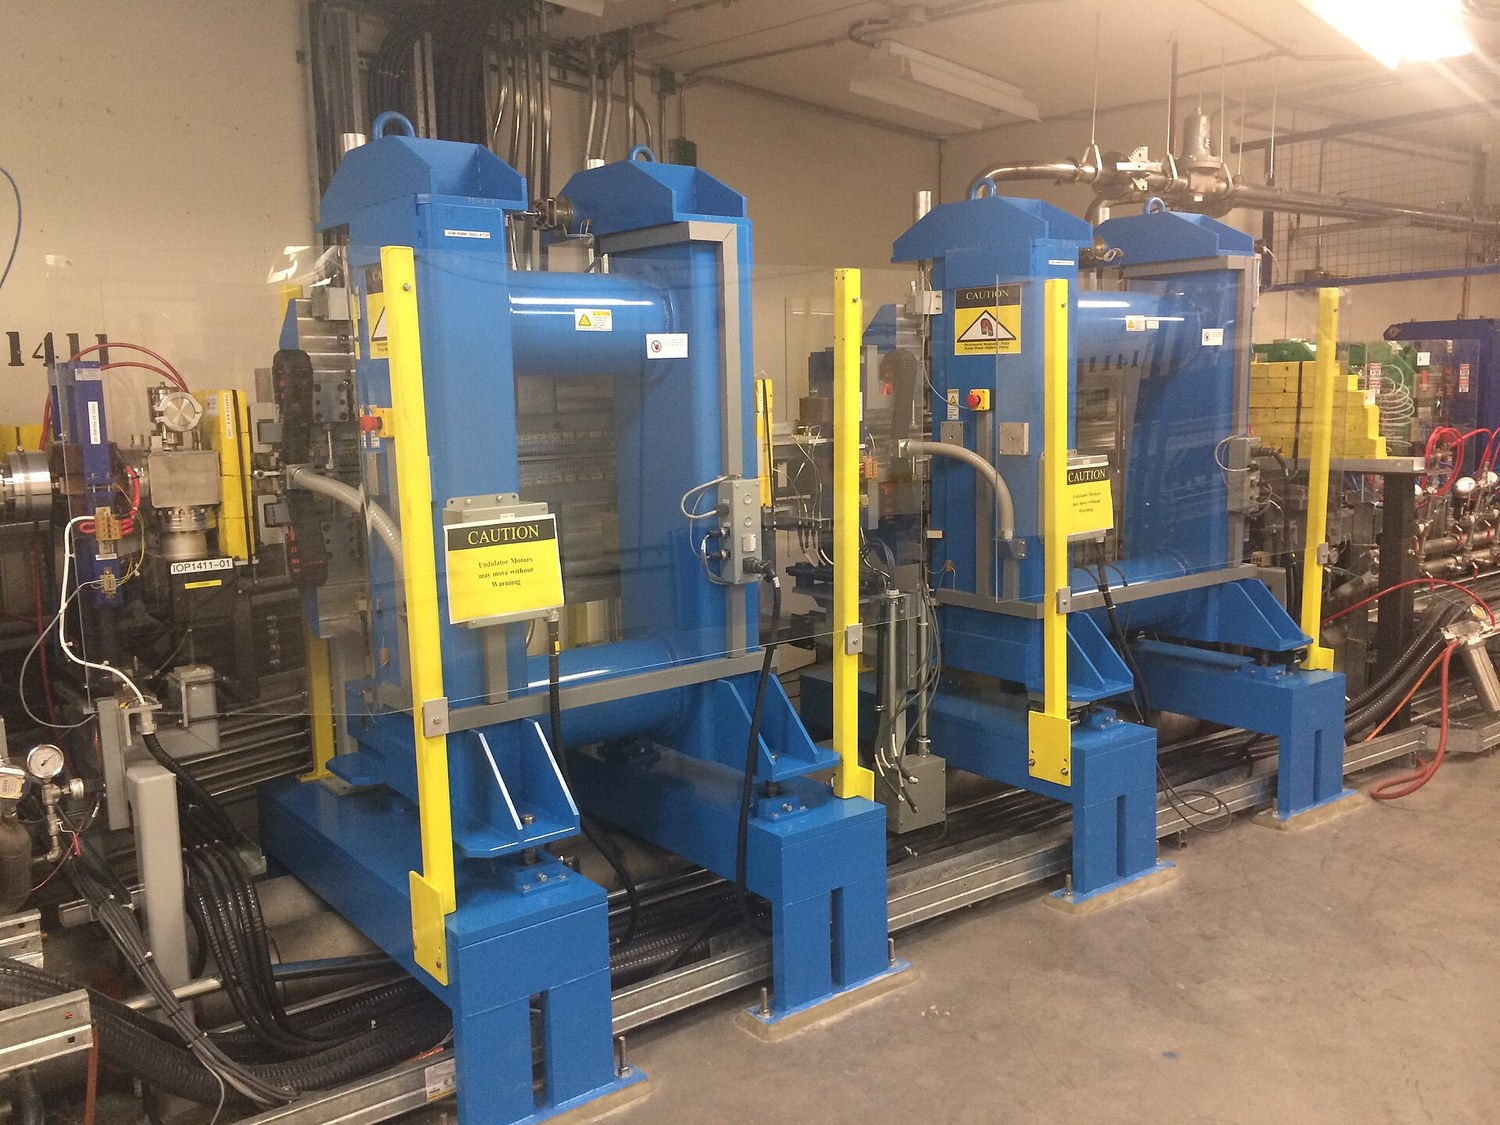
\includegraphics[width=0.72\textwidth]{../figures/x_storage_ring.jpg}
\caption{同步辐射储存环：回旋辐射从「损失」变成「工具」。本节把回旋辐射当损失算；把电子加速到相对论能量后，同一种辐射成了同步辐射光源——同一套公式，两种用法。}
\label{fig:photo-appx2}
\figsource{CLS Research Office，CC BY-SA 2.0（Wikimedia Commons）}
\end{figure}

\section{回旋辐射：一个必须先谈输运的量}
\label{sec:app-x-cyclotron}

电子在磁场里做回旋运动，必然辐射。回旋频率是
\begin{equation}
f_{ce} = \frac{eB}{2\pi m_e} = 1.4836\times10^{11}\ \mathrm{Hz}
= 148.36\ \mathrm{GHz},
\label{eq:app-x-cyclfreq}
\end{equation}
单电子的 Larmor 功率（非相对论）是
\begin{equation}
P_1 = \frac{4}{3}\sigma_T c\,\beta_\perp^2\,u_B = 1.06947\times10^{-14}\ \mathrm{W},
\label{eq:app-x-larmor}
\end{equation}
代入 $\beta_\perp^2=0.035984$、$u_B=1.11767\times10^{7}\ \mathrm{J\,m^{-3}}$。
乘以电子密度 $n_e=10^{20}\ \mathrm{m^{-3}}$ 得光学薄功率密度
$1.06947\ \mathrm{MW\,m^{-3}}$，再乘 $V$ 得
\begin{equation}
P_{\mathrm{CYC}}^{\mathrm{thin}} = 890.01\ \mathrm{MW}
= 1.5993\,P_{\mathrm{fus}}.
\label{eq:app-x-cycthin2}
\end{equation}
这个数字不可能是真的（反应堆不能靠辐射损失掉 $160\%$ 的聚变功率），
所以必须问：逃逸份额到底是多少？

另一个边界是黑体上限。若等离子体对自己的回旋辐射完全黑体，
逃逸通量由 Rayleigh--Jeans 极限给出（$h\nu\ll k_BT$ 当然成立：
$h\nu/k_BT=6.6736\times10^{-8}$），按一个谐波带宽 $\sim f_{ce}$ 估：
\begin{equation}
F_{\mathrm{RJ}} = \frac{2\pi\nu^3 k_BT}{c^2}
= 336.283\ \mathrm{W\,m^{-2}},
\qquad
P_{\mathrm{CYC}}^{\mathrm{bb}} = F_{\mathrm{RJ}}\,A = 0.164622\ \mathrm{MW},
\label{eq:app-x-cycbb}
\end{equation}
其中第一壁面积取 $A=4\pi^2Ra=489.532\ \mathrm{m^2}$。于是
\begin{equation}
\frac{P_{\mathrm{CYC}}^{\mathrm{thin}}}{P_{\mathrm{CYC}}^{\mathrm{bb}}}
= 5406.41,
\qquad
\frac{P_{\mathrm{CYC}}^{\mathrm{bb}}}{P_{\mathrm{BR}}} = 0.60971\%.
\label{eq:app-x-supp}
\end{equation}
再吸收把光学薄上限压低了 $5406.41$ 倍，压到轫致辐射的 $0.60971\%$。
真值在 $0.164622\ \mathrm{MW}$ 与 $890.01\ \mathrm{MW}$ 之间，
具体是多少需要解辐射输运方程（含共振吸收、谐波重叠、壁反射），
\textbf{本附录不给这个数}——给的是两个边界，以及「为什么不能只用发射率」这个结论。

\begin{tip}{声明的量要写在明处}{tip-app-x-declared}
本节用到一个并不精确的量：谐波带宽取 $\sim f_{ce}$。
真实谐波线宽由多普勒展宽与相对论展宽决定，可以比 $f_{ce}$ 小一两个数量级，
那会把 $P_{\mathrm{CYC}}^{\mathrm{bb}}$ 同比例压低。把这类\textbf{估法本身}写在正文里，
而不是藏进系数，读者才能判断结论的适用范围。全书口径与附录 V 的
「把简化声明写在明处」一致。
\end{tip}

\begin{table}[htbp]
\centering
\small
\begin{tabular}{p{4.4cm}p{3.4cm}p{4.8cm}}
\toprule
量 & 数值 & 说明 \\
\midrule
回旋频率 $f_{ce}$ & $148.36\ \mathrm{GHz}$ & 式 \eqref{eq:app-x-cyclfreq} \\
磁能密度 $u_B$ & $1.11767\times10^{7}\ \mathrm{J\,m^{-3}}$ & $B^2/(2\mu_0)$ \\
单电子功率 $P_1$ & $1.06947\times10^{-14}\ \mathrm{W}$ & 式 \eqref{eq:app-x-larmor} \\
光学薄功率密度 & $1.06947\ \mathrm{MW\,m^{-3}}$ & 上限，偏大 \\
光学薄总量 & $890.01\ \mathrm{MW}$ & $=1.5993\,P_{\mathrm{fus}}$，不可能 \\
黑体通量 $F_{\mathrm{RJ}}$ & $336.283\ \mathrm{W\,m^{-2}}$ & 式 \eqref{eq:app-x-cycbb} \\
黑体总量 & $0.164622\ \mathrm{MW}$ & 下限，偏小 \\
再吸收压低倍数 & $5406.41$ & 上下限之比 \\
黑体上限占轫致辐射 & $0.60971\%$ & 结论：回旋不是主要损失 \\
\bottomrule
\end{tabular}
\caption{回旋辐射的两个边界。真值夹在第七行与第五行之间，
本附录不给输运方程的解；表的作用是把「不可能」与「可忽略」同时钉住。}
\label{tab:app-x-cyclotron}
\end{table}

{\footnotesize
\textbf{出处：}回旋辐射的单粒子功率、谐波结构与电子回旋波的输运处理参照
Bornatici 等（1983）\emph{Nucl.\ Fusion} \textbf{23}, 1153 与
Hutchinson \emph{Principles of Plasma Diagnostics}（2002，第 6 章）。
Rayleigh--Jeans 极限参照 Rybicki \& Lightman（1979，第 1 章）。
}

\section{线辐射与杂质：辐射崩塌}
\label{sec:app-x-line}

杂质离子的束缚-束缚跃迁给出线辐射，功率密度写成
\begin{equation}
P_{\mathrm{line}} = n_e n_{\mathrm{imp}} L_z(T_e),
\label{eq:app-x-line2}
\end{equation}
其中 $L_z$ 是冷却率系数，对每一种杂质是温度的函数。
取钨、$n_W/n_e=10^{-5}$（即 $n_W=10^{15}\ \mathrm{m^{-3}}$），
并取 $L_W(10\ \mathrm{keV})=10^{-32}\ \mathrm{W\,m^3}$ 的量级值，得
$P_{\mathrm{line}}=1\ \mathrm{kW\,m^{-3}}$、$P_{\mathrm{LINE}}=0.8322\ \mathrm{MW}$，
只占轫致辐射的 $3.08222\%$。也就是说，\textbf{在芯部温度上，钨并不构成威胁}。

真正的危险来自「多少杂质算太多」。令线辐射等于 alpha 自加热功率，
得到辐射崩塌阈值
\begin{equation}
n_W^{*} = \frac{P_\alpha}{V n_e L_W} = 1.3374\times10^{17}\ \mathrm{m^{-3}},
\qquad
\frac{n_W^{*}}{n_e} = 0.133742\%.
\label{eq:app-x-collapse}
\end{equation}
注意这个阈值是\textbf{按芯部温度}算的，而 $L_z(T)$ 在低温端高得多：
杂质冷却率曲线在几十到几百 eV 处有峰值，那里 $L_z$ 可以比 $10\ \mathrm{keV}$
处高一到三个数量级。所以杂质约束的真正瓶颈不在芯部，在\textbf{边界}——
这正是附录 N 讲杂质输运与脱靶时反复出现的那条结论，
本附录只是把它的定量理由补上。

\begin{tip}{「本附录只给上下限，不给输运方程的解」}{tip-app-x-honest}
本附录有意留下两个未定量的地方：回旋辐射的真实逃逸份额（只给两个边界）、
杂质冷却率曲线在边界温度上的具体数值（只给量级与趋势）。
这两处都需要本附录没有引入的工具：辐射输运方程与原子物理数据库。
把做不到的地方标出来，比用一个看起来精确的数字盖过去更有用：
前者的误差是已知的，后者的误差是隐藏的。
\end{tip}

\begin{table}[htbp]
\centering
\small
\begin{tabular}{p{2.8cm}p{3.2cm}p{3.2cm}p{3.4cm}}
\toprule
杂质 & $L_z$ 峰值温度 & 峰值相对高低 & 主要影响区 \\
\midrule
碳、氧（低 $Z$） & 十几到几十 eV & 高 & 边界、脱靶 \\
氩、氖（中 $Z$） & 百 eV 量级 & 很高 & 偏滤器辐射制冷 \\
钨（高 $Z$） & 千 eV 量级 & 高 & 芯部积累才是威胁 \\
\bottomrule
\end{tabular}
\caption{杂质冷却率曲线的形状（\textbf{定性}：只给峰值温度区间与相对高低，
不给具体数值，因为本附录没有引入原子物理数据库）。本表的用途是判断
「哪一种杂质在哪一个温度区间最危险」，与表 \ref{tab:app-x-budget} 配合使用。}
\label{tab:app-x-impurity}
\end{table}

{\footnotesize
\textbf{出处：}冷却率系数的定义与杂质辐射崩塌的图像参照 Post 等（1977）
\emph{At.\ Data Nucl.\ Data Tables} \textbf{20}, 397 与 ADAS 数据库的公开说明。
钨在 $10\ \mathrm{keV}$ 的量级取值按上述来源的曲线读数量级，具体精度不声明。
}

\begin{figure}[htbp]
\centering
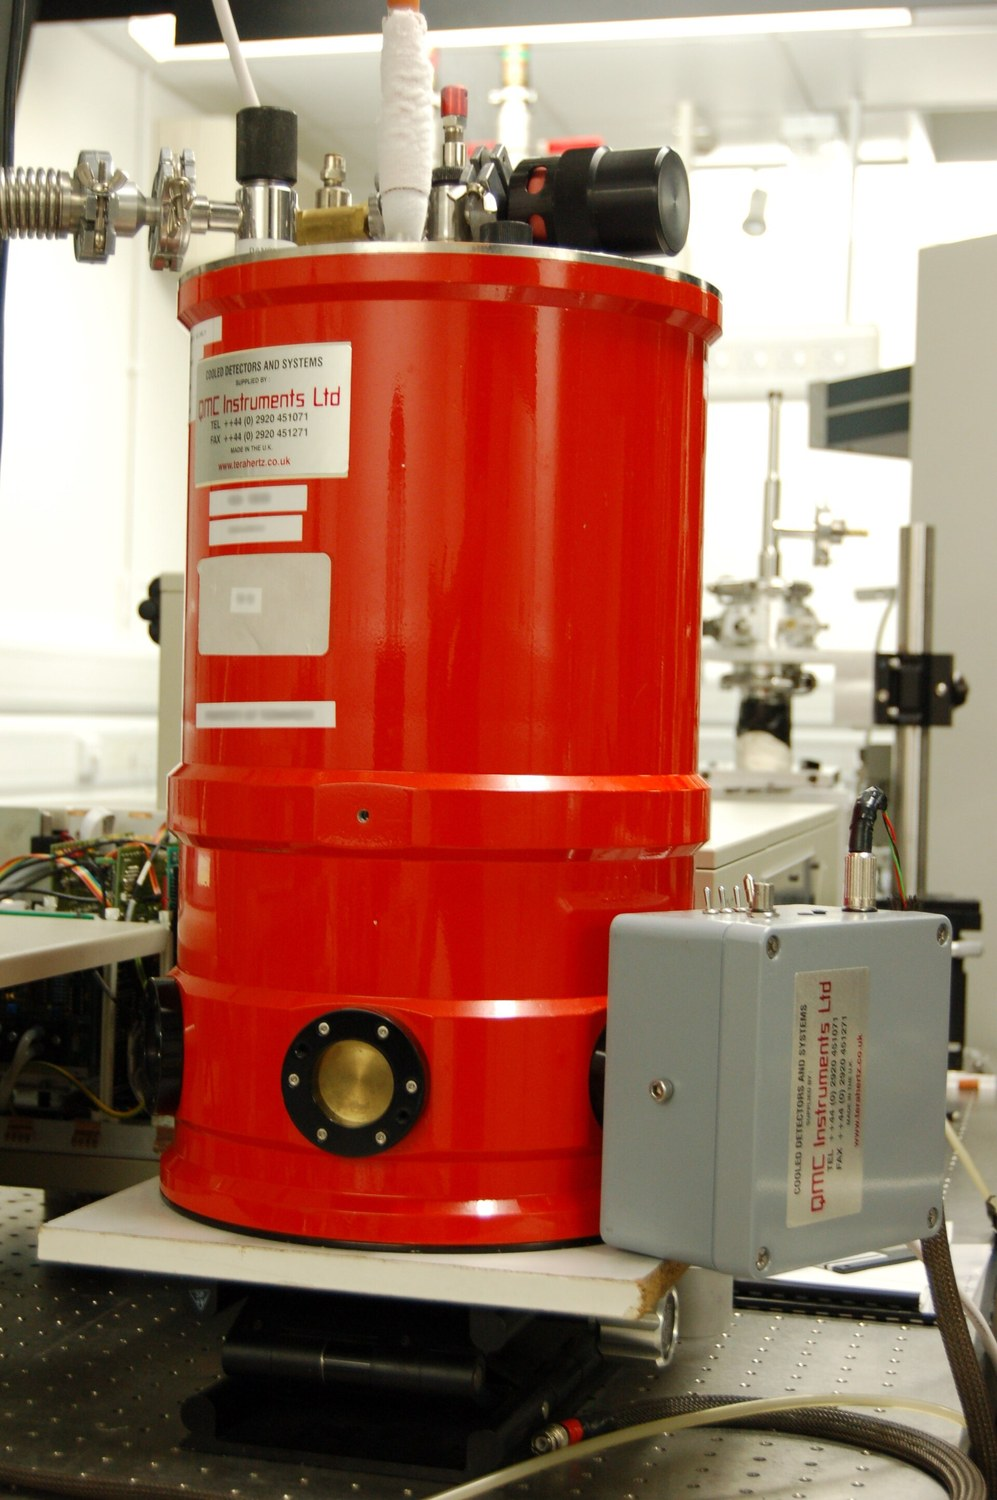
\includegraphics[width=0.52\textwidth]{../figures/x_bolometer.jpg}
\caption{辐射热计：吸收体把入射辐射变成温升，再由电桥读出——聚变装置里算辐射损失，靠的就是这类探测器。本节最后要把它放回功率账：辐射掉了多少，剩下的才轮到输运。}
\label{fig:photo-appx3}
\figsource{Alkamid，CC BY-SA 3.0（Wikimedia Commons）}
\end{figure}

\section{辐射在功率账里的位置}
\label{sec:app-x-budget}

把两笔主要辐射损失加起来：
\begin{equation}
P_{\mathrm{rad}} = P_{\mathrm{BR}} + P_{\mathrm{LINE}}
= 27.8322\ \mathrm{MW}
= 5.00129\%\,P_{\mathrm{fus}},
\label{eq:app-x-prad}
\end{equation}
而自加热余量是
\begin{equation}
\frac{P_\alpha}{P_{\mathrm{rad}}} = 3.99897,
\label{eq:app-x-margin}
\end{equation}
也就是大约 \textbf{4 倍，不是 100 倍}。
在 D1 这种「点火裕度看起来不错」的工作点上，
alpha 自加热有四分之一被辐射直接带走，
剩下三倍于辐射损失的余量才用来抵消输运损失。
附录 U 的三重积账若把辐射漏掉，$Q$ 会被高估。

辐射单独把热储能抽干需要
\begin{equation}
\tau_{\mathrm{rad}} = \frac{W_{\mathrm{th}}}{P_{\mathrm{rad}}}
= 13.3443\ \mathrm{s},
\label{eq:app-x-taurad}
\end{equation}
与附录 V 的电流猝灭时间 $\tau_{\mathrm{CQ}}=76.9074\ \mathrm{ms}$ 相比慢了
$173.511$ 倍——\textbf{辐射是慢刀子，破裂是快刀子}：前者决定稳态运行点能不能维持，
后者决定这个点在多快的时间里被拆掉。

\begin{table}[htbp]
\centering
\small
\begin{tabular}{p{3.0cm}p{3.0cm}p{3.2cm}p{4.2cm}}
\toprule
项目 & 数值 & 与 $P_\alpha$ 之比 & 含义 \\
\midrule
轫致辐射 $P_{\mathrm{BR}}$ & $27.00\ \mathrm{MW}$ & $24.2588\%$ & 光学薄，全部逃逸 \\
线辐射 $P_{\mathrm{LINE}}$ & $0.8322\ \mathrm{MW}$ & $0.747709\%$ & 钨 $10^{-5}$，芯部不构成威胁 \\
辐射合计 $P_{\mathrm{rad}}$ & $27.8322\ \mathrm{MW}$ & $25.0065\%$ & 吃掉落四分之一自加热 \\
自加热余量 & $3.99897$ & --- & 约 4 倍，不是 100 倍 \\
辐射冷却时间 & $13.3443\ \mathrm{s}$ & --- & 比 $\tau_{\mathrm{CQ}}$ 慢 $173.511$ 倍 \\
壁面轫致热流 & $55.1547\ \mathrm{kW\,m^{-2}}$ & --- & X 射线，需屏蔽而非冷却 \\
\bottomrule
\end{tabular}
\caption{辐射在 D1 功率账里的位置。第三列把每项折算成 $P_\alpha=111.3\ \mathrm{MW}$
的百分比，便于与附录 U 的自加热账直接对照。}
\label{tab:app-x-budget}
\end{table}

\begin{tip}{自加热余量 4 倍，不是 100 倍}{tip-app-x-margin}
初学者容易把「点火」想成一件门槛之外就一劳永逸的事。表 \ref{tab:app-x-budget}
说明不是：即使 $Q$ 很大，$P_\alpha$ 也要先付掉四分之一的辐射账，
剩下的才轮到输运。所以「提高 $Z_{\mathrm{eff}}$」是一件代价极高的事——
它同时放大轫致辐射（线性）与线辐射（线性），而这两项都从自加热里扣。
\end{tip}

{\footnotesize
\textbf{出处：}功率平衡的分类与点火条件参照 Freidberg
\emph{Plasma Physics and Fusion Energy}（2007，第 13 章）。
把辐射损失单列成账的做法与附录 U 一致，与破裂时间尺度的对比参照附录 V。
}

\section{估算练习}
\label{sec:app-x-problems}

\textbf{练习 1} 若把 $Z_{\mathrm{eff}}$ 从 $2$ 降到 $1.5$（更干净的等离子体），
而 $n_e$、$T_e$ 不变，$P_{\mathrm{BR}}$ 变成多少？

\textbf{练习 2} 若 $T_e$ 从 $9.194\ \mathrm{keV}$ 翻倍到约 $20\ \mathrm{keV}$，
$P_{\mathrm{br}}$ 的功率密度变成多少？

\textbf{练习 3} 需要多高的钨浓度 $n_W/n_e$，才能使线辐射等于轫致辐射？

\textbf{练习 4} 用黑体上限式 \eqref{eq:app-x-cycbb} 反推：若要让回旋辐射达到
$27.00\ \mathrm{MW}$，亮度温度需要多高？这个结果说明什么？

\textbf{练习 5} 自由-自由光学深度要变成 $1$，弦长需要多长？与装置尺度比是多少倍？

\textbf{练习 6} 若屏蔽层把 $27.00\ \mathrm{MW}$ 的轫致辐射全部吸收，
第一壁每平方米每秒沉积多少能量？与偏滤器稳态热流（约 $0.1\ \mathrm{MW\,m^{-2}}$）相比如何？

\textbf{解答 1} $P_{\mathrm{br}}\propto Z_{\mathrm{eff}}$，所以从 $27.00\ \mathrm{MW}$
降到 $27.00\times1.5/2=20.25\ \mathrm{MW}$。\textbf{要点}：只有轫致辐射按 $Z_{\mathrm{eff}}$
线性缩放，线辐射按杂质浓度缩放，两者机制不同。

\textbf{解答 2} $P_{\mathrm{br}}\propto\sqrt{T_e}$，比值
$\sqrt{20/9.194}=1.4749$，所以
$32.444\times1.4749=47.8519\ \mathrm{kW\,m^{-3}}$。\textbf{要点}：温度翻倍辐射只涨 $47.49\%$，
这解释了为什么提高温度是改善点火裕度的主要手段。

\textbf{解答 3} 令 $n_e n_W L_W = P_{\mathrm{BR}}/V$，得
$n_W = 3.24441\times10^{16}\ \mathrm{m^{-3}}$，即
$n_W/n_e = 0.0324441\%$。比式 \eqref{eq:app-x-collapse} 的崩塌阈值
$0.133742\%$ 低四倍多。\textbf{要点}：让线辐射追上轫致辐射所需浓度非常低，
所以「杂质辐射」这件事在芯部也不能完全无视。

\textbf{解答 4} 黑体上限正比于温度，故
$T = 1507.93\ \mathrm{keV}$，
即约 $1.5\ \mathrm{MeV}$——比实际温度高两个数量级多。
\textbf{要点}：黑体上限在本工作点上远小于轫致辐射，
说明回旋辐射即使被完全再吸收也不会成为主要损失。

\textbf{解答 5} $L = 1/\alpha_{ff} = 6.8301\times10^{5}\ \mathrm{m} = 683.011\ \mathrm{km}$，
是 $2a=4\ \mathrm{m}$ 的 $1.7075\times10^{5}$ 倍。\textbf{要点}：要让托卡马克对轫致辐射光学厚，
需要的尺度是千公里量级——恒星内部才满足，实验室等离子体永远光学薄。

\textbf{解答 6} $27.00\ \mathrm{MW}/489.532\ \mathrm{m^2}=55.1547\ \mathrm{kW\,m^{-2}}
=0.0551547\ \mathrm{MW\,m^{-2}}$，约为偏滤器稳态热流的一半。
\textbf{要点}：数值上不大，但它是穿透性 X 射线、不被磁场偏转，
所以对材料的要求不是「耐热」而是「屏蔽」——见 X.3 的提示盒。

\section{来源、分级与版权说明}
\label{sec:app-x-source}

\begingroup\small
本附录按难度分三档：X.1 与 X.2 是量级与判据，X.3 与 X.4 是两种机制的具体算法，
X.5 与 X.6 是把辐射放回功率账。练习 1--6 只需要本附录的公式与表，不需要查外部数据。

\begin{table}[htbp]
\centering
\small
\begin{tabular}{p{3.4cm}p{5.6cm}p{3.6cm}}
\toprule
本附录内容 & 借鉴来源 & 在本书里的位置 \\
\midrule
轫致辐射公式与 $Z_{\mathrm{eff}}$、$\sqrt{T_e}$ 依赖 &
Wesson \emph{Tokamaks}（第 4 版，2011）第 2 章；NRL \emph{Plasma Formulary}（2018） &
附录 U 的辐射损失行、本附录 X.3 \\
光学深度与自由-自由吸收 &
Rybicki \& Lightman \emph{Radiative Processes in Astrophysics}（1979）第 1、5 章 &
本附录 X.2 \\
回旋辐射、共振吸收与电子回旋波 &
Bornatici 等（1983）\emph{Nucl.\ Fusion} \textbf{23}, 1153；Hutchinson（2002）第 6 章 &
附录 Q 的电子回旋诊断、本附录 X.4 \\
杂质冷却率曲线与辐射崩塌 &
Post 等（1977）\emph{At.\ Data Nucl.\ Data Tables} \textbf{20}, 397；ADAS 数据库 &
附录 N 的杂质输运、本附录 X.5 \\
功率平衡与点火条件 &
Freidberg \emph{Plasma Physics and Fusion Energy}（2007）第 13 章 &
附录 U、本附录 X.6 \\
第一壁热流与屏蔽口径 &
与附录 N 同一套口径（本书自拟的账） &
附录 N、本附录 X.3 \\
\bottomrule
\end{tabular}
\caption{本附录的借鉴来源与对应位置。只借鉴物理结论、公式形式与题型；
全部数值、表格与文字自拟并由仓库脚本复算。}
\label{tab:app-x-source}
\end{table}

版权与复现口径，四条：第一，\textbf{不复制}任何教材或论文的表格数值，
表 \ref{tab:app-x-channel} 到表 \ref{tab:app-x-source} 的每一个数字都由
\texttt{tools/\allowbreak{}calc/\allowbreak{}appX\_calc.py} 在给定工作点上现算；第二，\textbf{不复制}原书的题面与解答文字，
练习 1--6 的题目与解答均为本书自拟；第三，\textbf{不复制}无法核验的 DOI 编号，
一律只给书名、作者、年份、卷期页；第四，\textbf{不复制}任何未经复算的「精确值」——
凡本附录引入的\textbf{声明值}（钨的冷却率系数 $10^{-32}\ \mathrm{W\,m^3}$、
回旋谐波带宽 $\sim f_{ce}$）都在正文里写明是量级值，不假装精确。
\endgroup
